\section{Iteration \#2 -- Pseudo-Pyramid Tree Optimisation}

In the first iteration, the Pseudo-Pyramid Tree showed great promise as an efficient index structure for high-dimensional data. The core limitation of the implementations was that \texttt{delete} operations were dramatically slower than other operations because of its worst case complexity of $O(n^2)$ if memory must be released. This iteration focuses on modifying the Pseudo-Pyramid Tree in attempt to maintain the good performance of \texttt{insert} and point queries, but increase \texttt{delete} speed. Iteration 2's objectives are:
\begin{itemize}
	\item Implement variant of the Pseudo-Pyramid Tree based on rebuilding the structure to defragment
	\item Implement non-index based Pseudo-Pyramid Tree
	\item Implement Splay tree and Splay Pseudo-Pyramid Tree, which uses splay tree as one-dimensional back-end
	\item Fine-tune and optimise the implementations using knowledge about the test environment/hardware
	\item Analyse performance of all Pseudo-Pyramid Tree variants and determine the best performing one
\end{itemize}

\subsection{Accelerating Hash Function}

It was shown in the last iteration that the Pseudo-Pyramid tree eventually becomes slower than Sequential Scan as $d$ increases. Since the plots showed the increase in the Pseudo-Pyramid Tree's execution time is roughly quadratic, and the structure spend most of that time in the $O(d^2)$ hashing function (Equation \ref{eq:pseudo-pyramid-hash}), it follows that speeding up the hashing function would provide large speed gains.

The existing point hashing function takes $O(d^2)$ time because of the inner loop that computes $\prod_{j=0}^{i}{\lbrack m_j \rbrack}$. If $m$ is changed during the structure's lifetime. otherwise the hash value of a point could change and stored points can become inaccessible. Therefore, $m$ is constant and the hashing function can computed in $O(d)$ time by \textit{pre-computing} $\prod_{j=0}^{i}{\lbrack m_j \rbrack}$. This pre-computation happens when the Pseudo-Pyramid tree is initialised. The new hashing function is given in Equation \ref{eq:new-pseudo-pyramid-hash}.

\begin{multline}\\
	h(p) = \sum_{i = 0}^{d} { \lbrack \texttt{toInt}( h_i(p) \times m_i ) \times M_i \rbrack } \\
	\text{where } M_i = \prod_{j=0}^{i}{\lbrack m_j \rbrack} \;\;\; \text{for} \; 0 \leq i \leq d \\
	\label{eq:new-pseudo-pyramid-hash}
\end{multline}

Table \ref{tab:new-pseudo-pyramid-hash} shows operation execution time of the Batch Pyramid Tree using the original $O(d^2)$ hashing function and the new $O(d)$ function. The tes used the Insert-Query-Remove operation list on the uniform synthetic dataset with 200 dimensions. Figure \ref{fig:new-pseudo-pyramid-hash} plots the performance of the Pseudo-Pyramid tree with both hash functions alongside Sequential Scan, showing execution time against dimensionality. From the plot, it is clear that the new hashing function provides superior speed; the Pseudo-Pyramid Tree is now significantly faster than Sequential Scan, even for dimensions as high as 200.

\begin{table}
	\centering
	\begin{tabular}{|l|l|l|}
		\hline
		\textbf{Operation} & \textbf{$O(d^2)$ Function} & \textbf{$O(d)$ Function} \\
		\hline
		\textbf{Insert} & 1.46412 & 0.0112199 \\
		\textbf{Delete} & 0.730777 & 0.00625336 \\
		\textbf{Point Query} & 0.731469 & 0.0076015 \\
		\hline
	\end{tabular}
	\caption{Total Execution Time (in Seconds) of Batch Pseudo-Pyramid Tree Using $O(d^2)$ and $O(d)$ Hash Function (200D Randomly Uniform Dataset, 10,000 operations each)}
	\label{tab:new-pseudo-pyramid-hash}
\end{table}

\begin{figure}
	\centering
	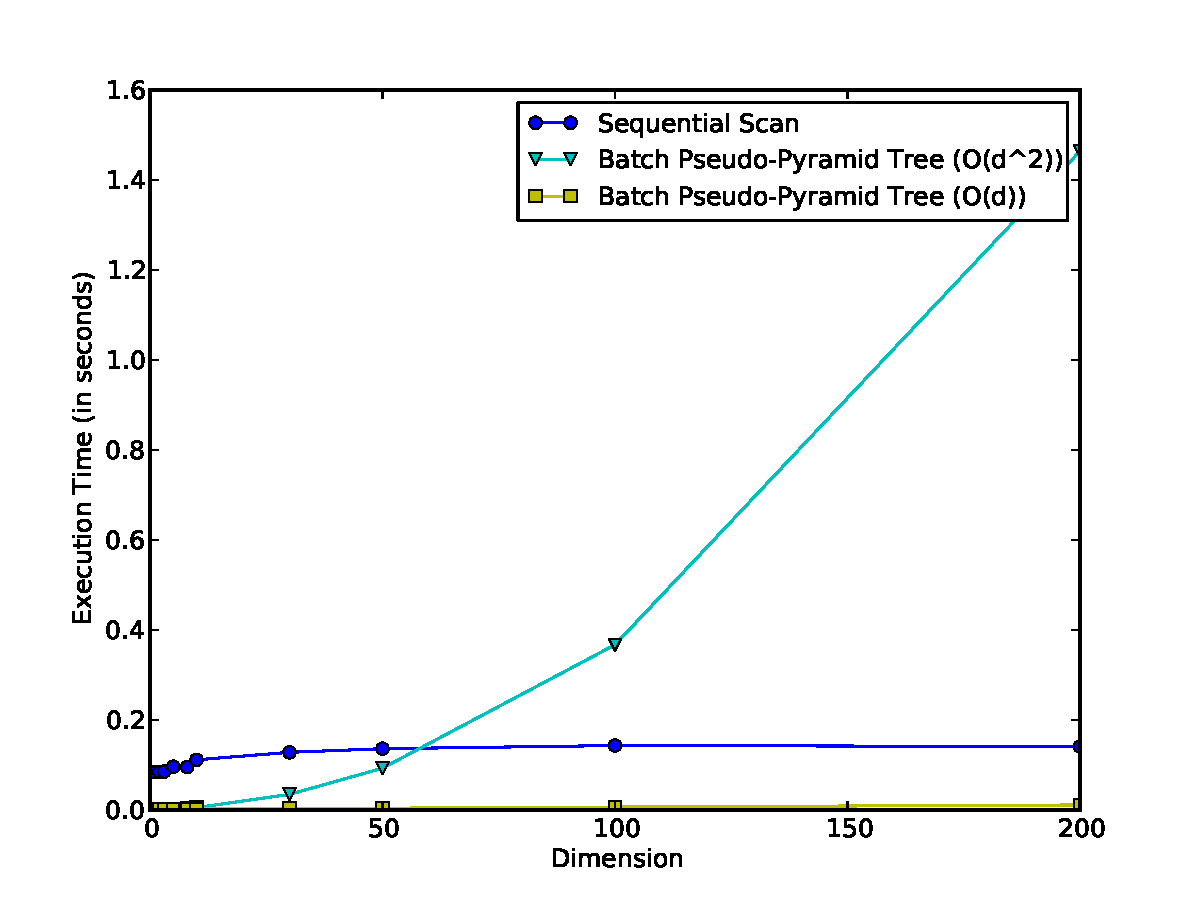
\includegraphics[scale=0.5]{figures/performance_analysis/iteration_2/new_pseudo-pyramid_hash_performance.pdf}
	\caption{\texttt{insert} Performance on Random Uniformly Distributed Datasets of Varying Dimensions}
	\label{fig:new-pseudo-pyramid-hash}
\end{figure}

\subsection{Improving Bucket Utlisation}

TODO: define what this is and how it can affect perform (too low, random access, too high, too many points to seach per query)

Define new hashign functions

TODO: State how this new function is easier to compute and provides better bucket utliisation -- BE SURE TO GIVE THE MEASUREMENTS FOR THIS TO PROVE IT! Discuss why bucket utilisation is better at a sweet spot (not too low, not too high)

TODO: discuss scaling factor, what it deos and why it can help (plots with scaling factor against bucket utilisation + execution time)

\subsection{SSE Parallelisation}

SIMD stands for Single Instruction, Multiple Data and was defined by Flynn as a classification of parallel computing \cite{flynns-taxonomy}. In SIMD, a single instruction is used to operation on multiple data items at the same time. If $p$ is the maximum number of data items that can be operated on in parallel at a time, then in an ideal scenario it is possible increase the speed of a computation by $p$ times. However, it is only suitable for computations where the same operation can be applied to multiple data items independantly, where the order in which those operations complete does not affect the final output.

Streaming SIMD Extensions, or SSE, is a specification of an instruction set that performs SIMD operations for the widely used x86 CPU architecture\cite{sse}, which is the architecture used for the development and test environment of this project. It was seen as TODO

TODO: speeding up NEW hashing function
TODO: speeding up point comparison

\subsection{Rebuild Pseudo-Pyramid Tree}

This variant of the Pseudo-Pyramid Tree uses a different strategy for releasing memory for unused points. Instead of defragmenting the array by peforming a sequence of array deletions when $R + 1$ elements are marked for deletion, the entire structure is rebuilt. This new cleanup procedure starts by clearing the structure and incrementally building the new structure by only adding points \textit{not} marked for deletion. $n - R$ points will be re-instered and insertion in the worst case is $O(n)$, meaning the worst case complexity of \texttt{delete} is $O((n - R)n)$. The larger $R$ is, the less time it takes to perform this procedure but a larger amount of allocated memory goes unused at a time.

\subsection{Bucket Pseudo-Pyramid Tree}

The Bucket Pseudo-Pyramid Tree implementation does not use a single array to store the points. Instead of buckets containing an array of point indices, it has an array of actual points. No clenaup procedure is necessary because the memory for a point is released immediately afer it's removed, by simply erasing it from the corresponding bucket's array. The goal of this is to increase \textbf{cache coherency} when searhcing a bucket, since the point array can be searched sequentially. The index-based variants cause random accesses in the single point array (causing more cache misses) since a bucket's store indices may point to distant parts of the point array, which may become very large.

% TODO: further explanation of cache misses?

Array deletion is a $O(n)$ operation since the case where a single bucket stores all $n$ points is possible, making \texttt{delete} $O(n)$ in the worst case. Since the order the points are stored in a bucket do not matter, the C++ \textit{erase-remove} idiom has been used to delete elements from the bucket arrays, which swaps the element to delete with the last element in the array, removing the desired element when it's at the end of the array. This prevents the required $O(n)$ shift operation which tightly pack the elements after a deletion.

\paragraph{\textbf{NOTE: }} From this point in the documentation onwards, all \texttt{std::vector} deletions where order does not matter will be performed using the erase-remove idiom.

\subsection{Splay Pseudo-Pyramid Tree}

Unlile the other implementations, the Splay Pseudo-Pyramid Tree does not use a hash map as the underyling one-dimensional index structure, but a splay tree. The splay tree is a self-adjusting variant of the binary search tree that uses a \textit{splaying} operation (a heuristic) to allow faster access to recently accessed elements. \cite{splay-tree}. The splaying operation achieves this by performing a series of tree rotations that move a given node up to the root of the tree. Through amortised analysis and empirical experiments, it has been shown splay trees can be more efficient than standard binary trees for a series of non-random operations \cite{splay-tree}, despite the asymptotic worst case bound being worse than binary search trees.

TODO: more detail about the splay tree, including in-depth algorithms??

Nodes in the Splay Pseudo-Pyramid Tree correspond to individual buckets in the Bucket Pseudo-Pyramid Tree, meaning each node can store multiple points. Since the splay tree is implemented as a collection of heap-allocated nodes with pointers to link them, deletions are cheap as a low amount of memory needs to be de-allocated per \texttt{delete} operation. The hope is that this, combined with the self-adjusting nature of the splay tree, will produce a Pseudo-Pyramid Tree implementation that is more efficient for non-random operations TODO.

\subsection{Parallelising Bucket Search}

TODO: thread pools and stuff. Differerent analyses

\subsection{Performance Analysis}

TODO: four structures
	Defragment Index Pseudo-Pyramid Tree
	Rebuild Index Pseudo-Pyramid Tree
	Bucket Pseudo-Pyramid Tree
	Splay Pseudo-Pyramid Tree

	R = 3000

TODO: justify WHY no-defrag (batch))Pseudo-Pyramid Tree is not being tested

TODO: refer to plots and justify why only there's only two here (rest are in appendices)

TODO: CPU/heap profiling

\begin{landscape}

	TODO: update tables in this

	\begin{table}
		\centering
		\begin{tabular}{|p{2cm}|l|l|l|l|l|l|l|l|l|l|l|}
			\hline
			\textbf{Structure} & \textbf{Operation} & \textbf{1D} & \textbf{2D} & \textbf{3D} & \textbf{5D} & \textbf{8D} & \textbf{10D} & \textbf{30D} & \textbf{50D} & \textbf{100D} & \textbf{200D} \\
			\hline
			\multirow{ 4}{*}{\textbf{Defragmented Index Pseudo-Pyramid Tree}} & \textbf{Insert} & 0.0100861 & 0.0110824 & 0.0125415 & 0.0150796 & 0.0198269 & 0.0243051 & 0.0977912 & 0.226317 & 0.793781 & 2.97191 \\
			 & \textbf{Delete} & 12.582 & 12.8934 & 12.9759 & 12.9543 & 12.8519 & 12.9391 & 13.1583 & 13.4074 & 14.2005 & 16.7081 \\
			 & \textbf{Point Query} & 0.0027684 & 0.00324225 & 0.00386536 & 0.00551307 & 0.00820208 & 0.0104848 & 0.049884 & 0.117446 & 0.408223 & 1.56195 \\
			\hline
			\multirow{ 4}{*}{\textbf{Rebuild Index Pseudo-Pyramid Tree}} & \textbf{Insert} & 0.0102503 & 0.0110619 & 0.0121741 & 0.0150467 & 0.0195684 & 0.0236087 & 0.0975364 & 0.226686 & 0.794168 & 2.98335 \\
			 & \textbf{Delete} & 12.5761 & 12.741 & 12.8164 & 12.8492 & 13.0039 & 13.0666 & 13.2909 & 13.582 & 14.5668 & 17.1137 \\
			 & \textbf{Point Query} & 0.00272942 & 0.00336814 & 0.00388157 & 0.00560772 & 0.00868261 & 0.0109097 & 0.0504385 & 0.117767 & 0.417613 & 1.54181 \\
			\hline
			\multirow{ 4}{*}{\textbf{Bucket Pseudo-Pyramid Tree}} & \textbf{Insert} & 0.015999 & 0.0172538 & 0.0181366 & 0.0208803 & 0.0257906 & 0.030085 & 0.103178 & 0.23306 & 0.798941 & 2.97632 \\
			 & \textbf{Delete} & 0.00354707 & 0.00423968 & 0.00467753 & 0.00626874 & 0.00936306 & 0.0119662 & 0.050822 & 0.120001 & 0.42113 & 1.52593 \\
			 & \textbf{Point Query} & 0.00234234 & 0.00291753 & 0.0036248 & 0.00529063 & 0.00801969 & 0.0101838 & 0.0508173 & 0.11813 & 0.413853 & 1.53966 \\
			\hline
			\multirow{ 4}{*}{\textbf{Splay Pseudo-Pyramid Tree}} & \textbf{Insert} & 0.0174001 & 0.0185397 & 0.0195724 & 0.0224078 & 0.0268705 & 0.0309955 & 0.104663 & 0.234407 & 0.799793 & 2.97659 \\
			 & \textbf{Delete} & 0.00412166 & 0.00481606 & 0.00533354 & 0.00767851 & 0.0102245 & 0.0132186 & 0.0525625 & 0.120654 & 0.424749 & 1.53488  \\
			 & \textbf{Point Query} & 0.00304317 & 0.00362563 & 0.0044601 & 0.00626445 & 0.00898099 & 0.0118438 & 0.0515605 & 0.119636 & 0.412084 & 1.53412 \\
			\hline
		\end{tabular}
		\caption{Execution Time (in Seconds) of 10,0000 Structure Operations for Uniformly Random Points}
		\label{tab:perf2-randuniform}
	\end{table}

	\begin{table}
		\centering
		\begin{tabular}{|r|l|l|}
			\hline
			\textbf{Structure} & \textbf{InsertAll-QueryAll-DeleteAll} & \textbf{10,000 Random Operations} \\
			\hline
			\textbf{Defragmented Index Pseudo-Pyramid Tree} & 126.073 & 61.1827 \\
			\textbf{Rebuild Index Pseudo-Pyramid Tree} & 127.648 & 60.9528 \\
			\textbf{Bucket Pseudo-Pyramid Tree} & 39.9721 & 17.872 \\
			\textbf{Splay Pseudo-Pyramid Tree} & 39.7724 & 17.9326 \\
			\hline
		\end{tabular}
		\caption{Execution Time (in Seconds) of Structures for Sampled Astrophysics Dataset}
		\label{tab:perf2-astrophysics}
	\end{table}

\end{landscape}

TODO: plot of insert() w/ skewed data
TODO: plot of delete() w/ rand uniform data

\subsection{Evaluation}

TODO
